%ID: 612059
\begin{center}

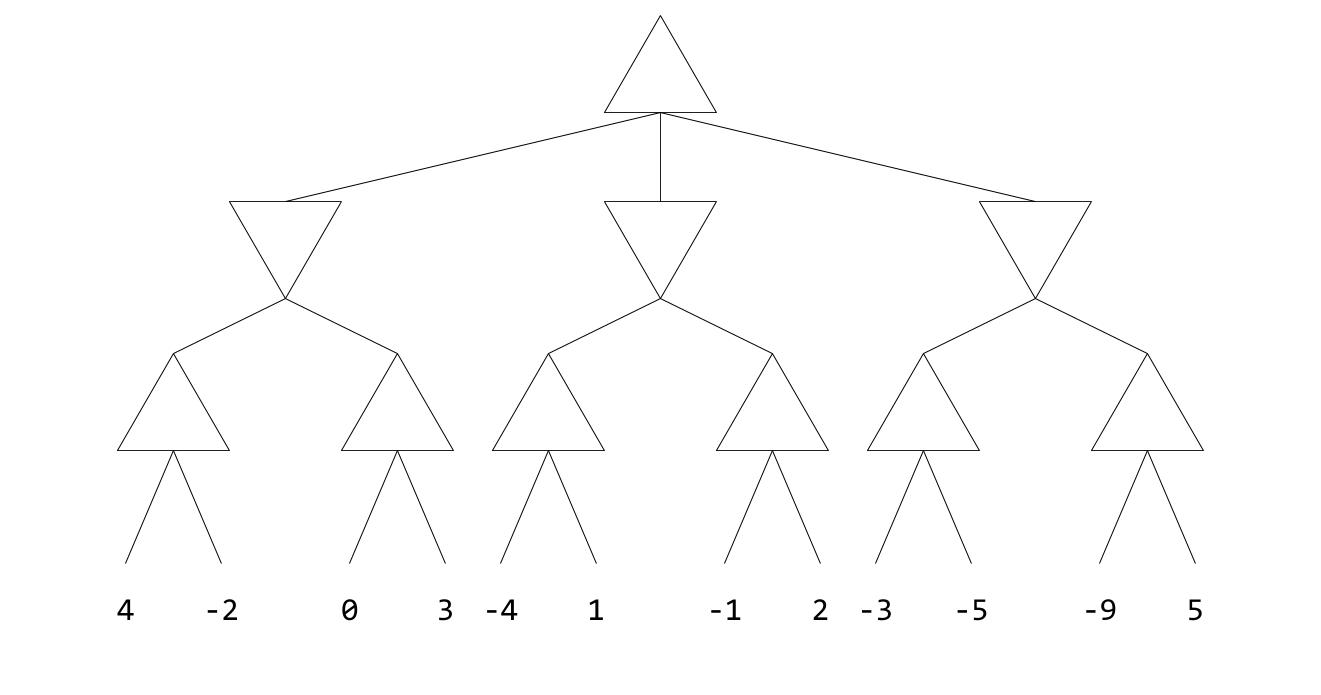
\includegraphics[scale=0.35]{topics/trees/game-trees/empty-alpha-beta.jpg}
\end{center}
\begin{enumerate}
\item Fill out the values in each ’maximizer’ and ’minimizer’ node for the above game tree after applying the Minimax algorithm to it.
\item Cross out (with an X) all branches that would be pruned by a Minimax implementation that utilizes alpha-beta pruning.
\ifprintanswers
\begin{solution}[2in]
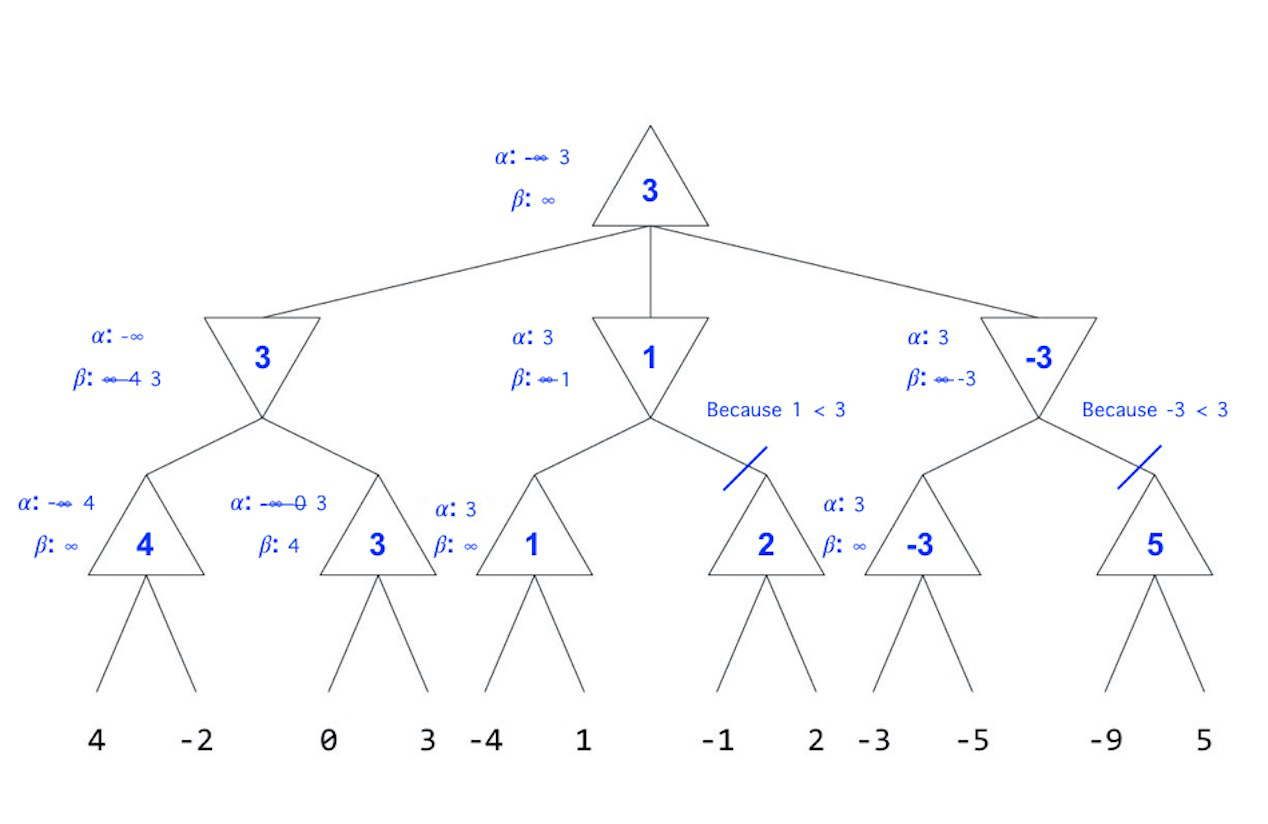
\includegraphics[scale=0.35]{topics/trees/game-trees/filled-alpha-beta.jpg}
$\alpha$ and $\beta$ values are updated every time a number returned from a child is either greater than $\alpha$ (for maximizer nodes) or less than $\beta$ (for minimizer nodes). \\
Pruning occurs between 1 and 2 in the center minimizer node because once the minimizer's value is updated to 1, 1 is less than $\alpha$ which is 3, so we know that the maximizer at the root will not choose 1 or anything less than 1 that the minimizer might return so we can prune the right child of the minimizer. We also prune between -3 and 5 in the rightmost minimizer for the same reason because $-3 < 3$.\\
\end{solution}
\fi
\item According to the Minimax algorithm, which move should we make for the above game?
\ifprintanswers
\begin{solution}[2in]
Go to the left sub-branch.
\end{solution}
\fi
\end{enumerate}